\documentclass[10pt, letterpaper]{article}

\usepackage{tikz} 
\usepackage{pgfplots}
\pgfplotsset{compat=1.9}
\usetikzlibrary{arrows,shapes,automata,backgrounds,petri,fit,decorations.pathmorphing, calc}

\begin{document}

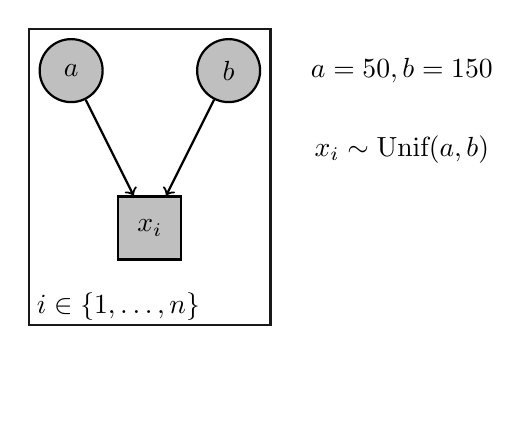
\begin{tikzpicture}[node distance = 2cm, double distance = 2pt, minimum size=.8cm, thick]
  \node[circle, draw=black, fill=lightgray] (a) {$a$};
  \node[circle, draw=black, fill=lightgray, right of=a] (b) {$b$};
  \node[rectangle, below of=a, draw=black, fill=lightgray, xshift = 1cm] (x) {$x_i$};
  
  \draw[->] (a)--(x);
  \draw[->] (b)--(x);
  
  \begin{pgfonlayer}{background}
      \node [thick,
             draw=black!90,fit={($(x.south)+(0,-20pt)$)
                                (a.west)
                                (a.north)
                                (b.east)}] {};
   \end{pgfonlayer}
    
   \node[below of=x] (TrialAnchor) {};
   \node[left of = TrialAnchor, xshift = 1.6cm, yshift = 1cm] (TrialLabel) {$i \in \{1, \ldots, n\}$};
   
   \begin{scope}[xshift = 4.2cm, node distance = 1cm]
       \node[] at(0, 0) (a) {$a = 50, b = 150$};
       \node[below of = a] (x) {$x_i \sim \mbox{Unif(}a, b)$};
    \end{scope}
    
\end{tikzpicture}

\end{document}